\chapter{Trave: SLE}
\section{Verifica tensioni massime di esercizio}
In questo paragrafo si affronta la verifica delle tensioni massime di esercizio per le sezioni della trave già precedentemente definite agli SLU, pertanto le caratteristiche geometriche e di armature sono le medesime.

Le ipotesi alla base di tale verifica riguardano la capacità di resistenza del calcestruzzo: esso infatti non si considera resistente a trazione, ovvero è in stato 2.
Si ipotizza inoltre il comportamento lineare ed elastico di calcestruzzo e acciaio e con un coefficiente di omogeinizzazione $n = 15$.

In riferimento alle \norma{NTC18} al capitolo \normaref{4.1.2.2.5} si deve avere che le tensioni di esercizio siano minori di quelle resistenti.
Si farà riferimento alla combinazione rara e a quella quasi permanente, con le tensioni resistenti riportate all'inizio di questo documento, al capitolo \ref{chap:materiali}.

Infine le formule che seguiranno faranno riferimento alla nomenclatura visibile in figura \ref{fig:sle_convenzione}.

\begin{figure}[htb]
    \centering
    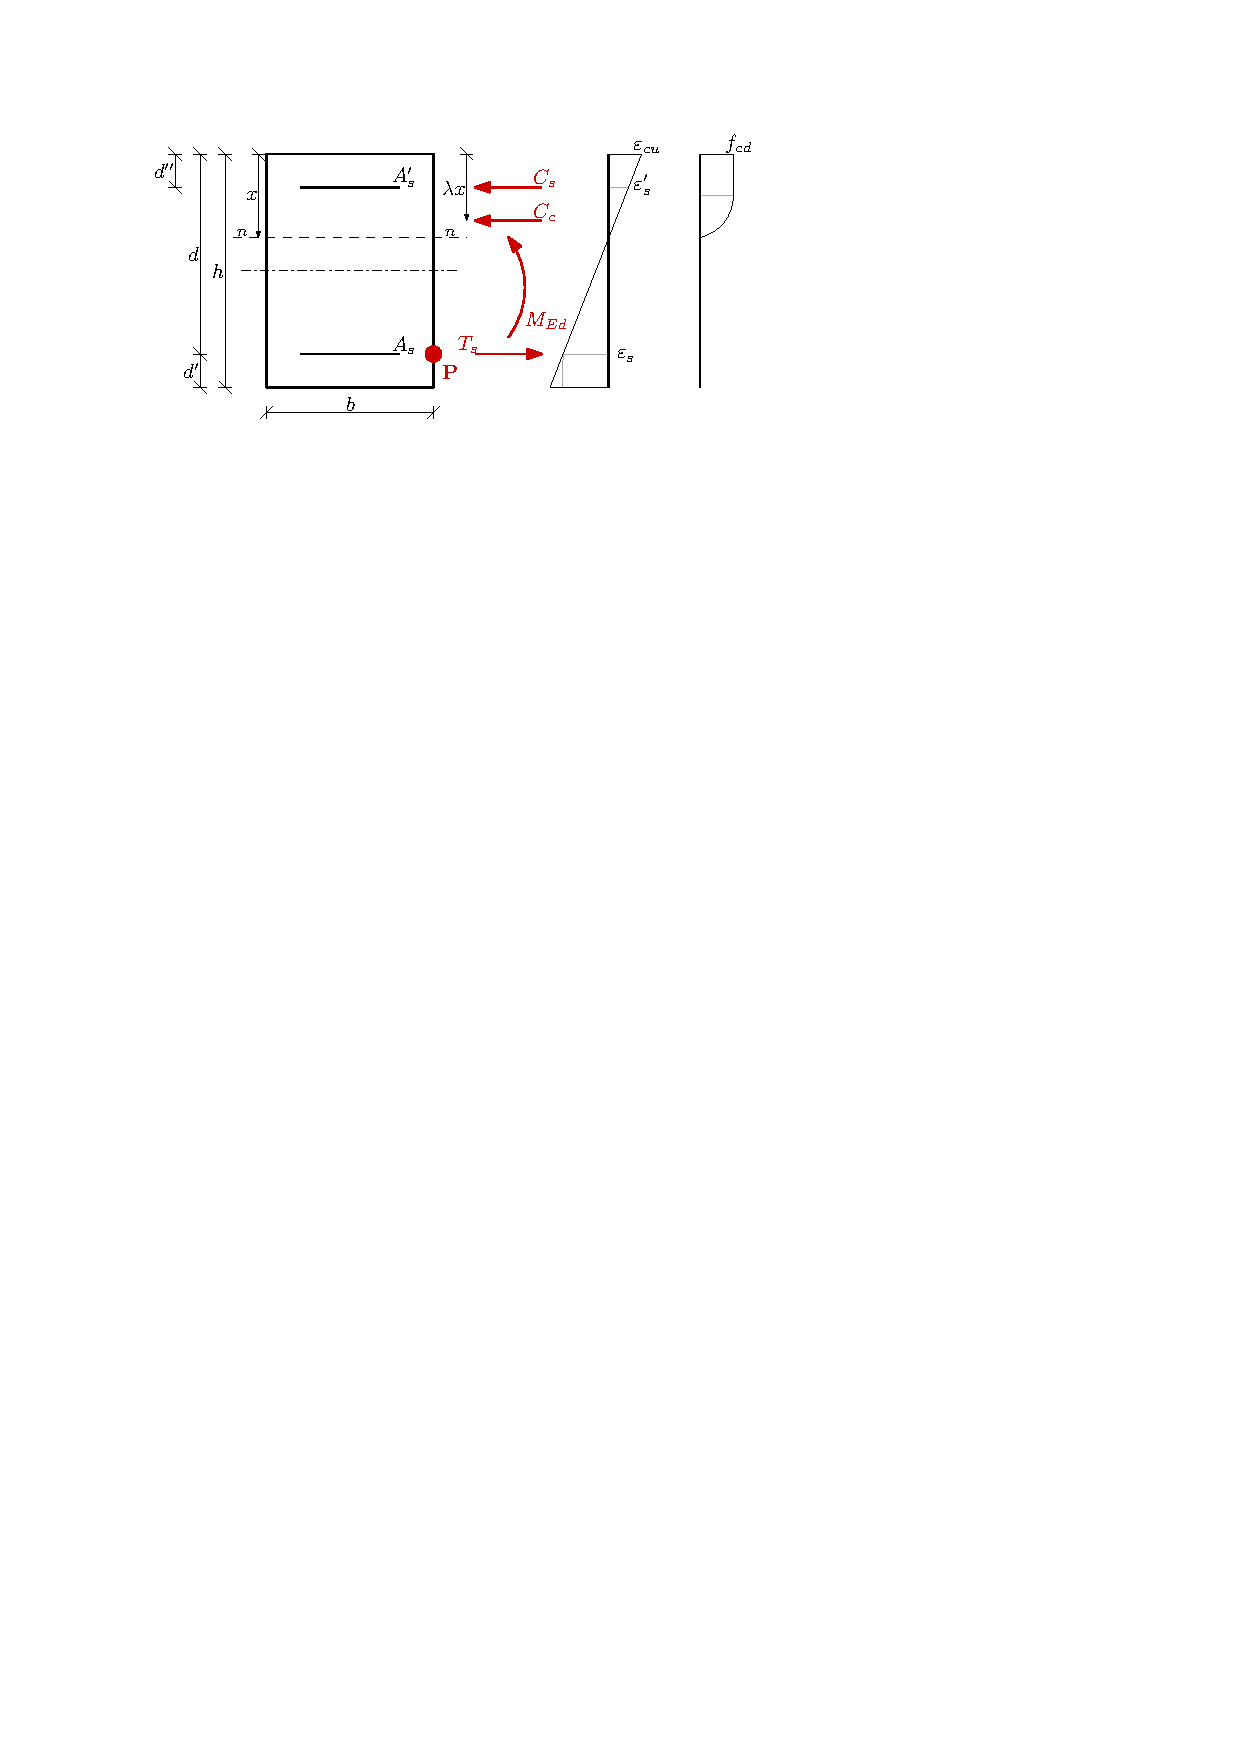
\includegraphics[height=0.25\textheight]{IMG/IPE_slu_progetto.pdf}
    \caption{Convenzione e nomenclatura utilizzata gli SLE}
    \label{fig:sle_convenzione}
  \end{figure}
  
Come primo passo occorre calcolare la posizione dell'asse netro $nn$ con la coordinata $x$. 
Per farlo è possibile risolvere il sistema di equilibrio alla traslazione e momento, oppure, in alternativa, essendo le azioni assiali nulle, si ha che il momento statico rispetto l'asse neutro è nullo. 
Da quest'ultima equazione è perciò possibile determinare $x$.
\begin{align}
    0 &= S_{nn}  \\
    0 &= \frac{1}{2} b\,x^2 + n\,A_s^\prime\,(x - d^{\prime\prime}) - n\,A_S(d-x) \\
    &\quad\hookrightarrow x = \frac{n\,(A_s^\prime + A_s)}{b} \left( -1 + \sqrt{1 + \frac{2\,b\,(A_s^\prime \, d^{\prime\prime} + A_s\,d)}{n\,(A_s^\prime + A_s)^2}} \, \right)
\end{align}
Trovata la posizione dell'asse neutro la tensione sul calcestruzzo la si ricava grazie all'equazione di Bernouli-Navier:
\begin{equation}
    \sigma_c = \frac{M_{Ed}}{I_{nn}} \, x
\end{equation}
dove $I_{nn}$ è riferito alla sezione reagente, pertanto si considera solo la zona compressa di calcestruzzo in aggiunta alle armature opportunamente omogeneizzate:
\begin{equation}
    I_{nn} = \frac{b\, x^3}{12} + n\,A_s^\prime\,(x - d^{\prime\prime})^2 - n\,A_s(d-x)^2 \quad.
\end{equation}
Infine le tensioni sull'acciaio si calcolano grazie alla linearità del diagramma delle tensioni:
\begin{align}
    \sigma_s &= \frac{n\,\sigma_c}{x} \, (d-x) \\
    \sigma_s^\prime &= \frac{n\,\sigma_c}{x} \,(x - d^{\prime\prime})
\end{align}

Tale procedimento è stato applicato per ogni sezione e i risultati sono visibili nelle tabelle \ref{tab:SLE_verifica_CHAR} e \ref{tab:SLE_verifica_QP}, rispettivamente per la combinazione rara e per quella quasi permanente.
Come si può notare la verifica è soddisfatta in tutte le sezioni.
\begin{table}[H]
    \centering
    \scriptsize
    \caption{SLS CHAR con $\sigma_c = \SI{15.00}{\mega\pascal}$ e $\sigma_s = \sigma_s^\prime = \SI{360.00}{\mega\pascal}$}
    \label{tab:SLE_verifica_CHAR}
    \begin{tabular}{
        l
        c
        c
        S[table-format=3.3]
        S[table-format=3.2]
        S[table-format=2.2]
        S[table-format=3.2]
        S[table-format=3.2]
        c
        c
        c}
    \toprule
    \multirow{2}{*}{Sez.} & \multirow{2}{*}{$A_s$} & \multirow{2}{*}{$A_s^\prime$} & {$M_{Ed}$} 				             & {$x$}                 & {$\sigma_c$}          & {$\sigma_s$}          & {$\sigma_s^\prime$}   & \multicolumn{1}{c}{\multirow{2}{*}{$\sigma_c<\sigma_{cR}$}}& \multicolumn{1}{c}{\multirow{2}{*}{$\sigma_s<\sigma_{sR}$}}& \multicolumn{1}{c}{\multirow{2}{*}{$\sigma_s^\prime<\sigma_{sR}^\prime$}} \\


                        &                        &                               & {\si{[\kilo\newton\metre]}} 			& {\si{[\milli\metre]}} & {\si{[\mega\pascal]}} & {\si{[\mega\pascal]}} & {\si{[\mega\pascal]}} &                                                   &                                                     &  \\
    \midrule
    A1 inv & 2Ø18 & 2Ø18 & 0.000   & 116.55 & 0.00  & 0.00   & 0.00   & \checked & \checked & \checked \\
    C1     & 3Ø18 & 2Ø18 & 52.840  & 139.36 & 4.83  & 166.84 & 51.70  & \checked & \checked & \checked \\
    A2 inv & 6Ø18 & 2Ø18 & 127.100 & 185.66 & 9.34  & 207.09 & 109.96 & \checked & \checked & \checked \\
    C2     & 4Ø18 & 2Ø18 & 93.640  & 157.51 & 7.79  & 224.43 & 87.18  & \checked & \checked & \checked \\
    A3 inv & 6Ø18 & 2Ø18 & 136.290 & 185.66 & 10.02 & 222.06 & 117.91 & \checked & \checked & \checked \\
    C3     & 3Ø18 & 2Ø18 & 65.970  & 139.36 & 6.04  & 208.30 & 64.55  & \checked & \checked & \checked \\
    A4 inv & 6Ø18 & 2Ø18 & 123.070 & 185.66 & 9.05  & 200.52 & 106.47 & \checked & \checked & \checked \\
    C4     & 4Ø18 & 2Ø18 & 81.210  & 157.51 & 6.76  & 194.64 & 75.61  & \checked & \checked & \checked \\
    A5 inv & 6Ø18 & 2Ø18 & 166.360 & 185.66 & 12.23 & 271.06 & 143.93 & \checked & \checked & \checked \\
    C5     & 4Ø18 & 2Ø18 & 103.770 & 157.51 & 8.63  & 248.71 & 96.61  & \checked & \checked & \checked \\
    A6 inv & 6Ø18 & 2Ø18 & 135.560 & 185.66 & 9.97  & 220.88 & 117.28 & \checked & \checked & \checked \\
    C6     & 2Ø18 & 2Ø18 & 27.760  & 116.55 & 2.93  & 129.60 & 28.88  & \checked & \checked & \checked \\
    A7 inv & 3Ø18 & 2Ø18 & 53.400  & 139.36 & 4.89  & 168.61 & 52.25  & \checked & \checked & \checked \\
    \midrule
    A1     & 2Ø18 & 2Ø18 & 0.000   & 116.55 & 0.00  & 0.00   & 0.00   & \checked & \checked & \checked \\
    C1 inv & 2Ø18 & 3Ø18 & 0.000   & 111.06 & 0.00  & 0.00   & 0.00   & \checked & \checked & \checked \\
    A2     & 2Ø18 & 6Ø18 & 0.000   & 97.91  & 0.00  & 0.00   & 0.00   & \checked & \checked & \checked \\
    C2 inv & 2Ø18 & 4Ø18 & 0.000   & 106.17 & 0.00  & 0.00   & 0.00   & \checked & \checked & \checked \\
    A3     & 2Ø18 & 6Ø18 & 0.000   & 97.91  & 0.00  & 0.00   & 0.00   & \checked & \checked & \checked \\
    C3 inv & 2Ø18 & 3Ø18 & 0.000   & 111.06 & 0.00  & 0.00   & 0.00   & \checked & \checked & \checked \\
    A4     & 2Ø18 & 6Ø18 & 0.000   & 97.91  & 0.00  & 0.00   & 0.00   & \checked & \checked & \checked \\
    C4 inv & 2Ø18 & 4Ø18 & 0.000   & 106.17 & 0.00  & 0.00   & 0.00   & \checked & \checked & \checked \\
    A5     & 2Ø18 & 6Ø18 & 0.000   & 97.91  & 0.00  & 0.00   & 0.00   & \checked & \checked & \checked \\
    C5 inv & 2Ø18 & 4Ø18 & 0.000   & 106.17 & 0.00  & 0.00   & 0.00   & \checked & \checked & \checked \\
    A6     & 2Ø18 & 6Ø18 & 0.000   & 97.91  & 0.00  & 0.00   & 0.00   & \checked & \checked & \checked \\
    C6 inv & 2Ø18 & 2Ø18 & 0.000   & 116.55 & 0.00  & 0.00   & 0.00   & \checked & \checked & \checked \\
    A7     & 2Ø18 & 3Ø18 & 0.000   & 111.06 & 0.00  & 0.00   & 0.00   & \checked & \checked & \checked \\
    \bottomrule
    \end{tabular}
    \end{table}
%%%%%%%%%%%%%%%%%%%%%%%%%%%%%%%%%%%%%%%%%%%%%%%%%%%%%%%%%%%%%%%%%
\begin{table}[H]
    \centering
    \scriptsize
    \caption{SLS QP con $\sigma_c = \SI{11.25}{\mega\pascal}$ e $\sigma_s = \sigma_s^\prime = \SI{360.00}{\mega\pascal}$}
    \label{tab:SLE_verifica_QP}
    \begin{tabular}{
        l
        c
        c
        S[table-format=3.3]
        S[table-format=3.2]
        S[table-format=2.2]
        S[table-format=3.2]
        S[table-format=3.2]
        c
        c
        c}
    \toprule
    \multirow{2}{*}{Sez.} & \multirow{2}{*}{$A_s$} & \multirow{2}{*}{$A_s^\prime$} & {$M_{Ed}$}                      & {$x$}                 & {$\sigma_c$}          & {$\sigma_s$}          & {$\sigma_s^\prime$}   & \multicolumn{1}{c}{\multirow{2}{*}{$\sigma_c<\sigma_{cR}$}}& \multicolumn{1}{c}{\multirow{2}{*}{$\sigma_s<\sigma_{sR}$}}& \multicolumn{1}{c}{\multirow{2}{*}{$\sigma_s^\prime<\sigma_{sR}^\prime$}} \\


                        &                        &                               & {\si{[\kilo\newton\metre]}}      & {\si{[\milli\metre]}} & {\si{[\mega\pascal]}} & {\si{[\mega\pascal]}} & {\si{[\mega\pascal]}} &                                                   &                                                     &  \\
    \midrule
    A1 inv & 2Ø18 & 2Ø18 & 0.000   & 116.55 & 0.00 & 0.00   & 0.00   & \checked & \checked & \checked \\
    C1     & 3Ø18 & 2Ø18 & 32.310  & 139.36 & 2.96 & 102.02 & 31.61  & \checked & \checked & \checked \\
    A2 inv & 6Ø18 & 2Ø18 & 89.860  & 185.66 & 6.61 & 146.41 & 77.74  & \checked & \checked & \checked \\
    C2     & 4Ø18 & 2Ø18 & 62.110  & 157.51 & 5.17 & 148.86 & 57.83  & \checked & \checked & \checked \\
    A3 inv & 6Ø18 & 2Ø18 & 94.390  & 185.66 & 6.94 & 153.79 & 81.66  & \checked & \checked & \checked \\
    C3     & 3Ø18 & 2Ø18 & 36.930  & 139.36 & 3.38 & 116.60 & 36.13  & \checked & \checked & \checked \\
    A4 inv & 6Ø18 & 2Ø18 & 84.390  & 185.66 & 6.20 & 137.50 & 73.01  & \checked & \checked & \checked \\
    C4     & 4Ø18 & 2Ø18 & 52.860  & 157.51 & 4.40 & 126.69 & 49.21  & \checked & \checked & \checked \\
    A5 inv & 6Ø18 & 2Ø18 & 128.520 & 185.66 & 9.45 & 209.40 & 111.19 & \checked & \checked & \checked \\
    C5     & 4Ø18 & 2Ø18 & 79.040  & 157.51 & 6.58 & 189.43 & 73.59  & \checked & \checked & \checked \\
    A6 inv & 6Ø18 & 2Ø18 & 105.910 & 185.66 & 7.79 & 172.57 & 91.63  & \checked & \checked & \checked \\
    C6     & 2Ø18 & 2Ø18 & 19.710  & 116.55 & 2.08 & 92.02  & 20.51  & \checked & \checked & \checked \\
    A7 inv & 3Ø18 & 2Ø18 & 33.500  & 139.36 & 3.06 & 105.77 & 32.78  & \checked & \checked & \checked \\
    \midrule
    A1     & 2Ø18 & 2Ø18 & 0.000   & 116.55 & 0.00 & 0.00   & 0.00   & \checked & \checked & \checked \\
    C1 inv & 2Ø18 & 3Ø18 & 0.000   & 111.06 & 0.00 & 0.00   & 0.00   & \checked & \checked & \checked \\
    A2     & 2Ø18 & 6Ø18 & 0.000   & 97.91  & 0.00 & 0.00   & 0.00   & \checked & \checked & \checked \\
    C2 inv & 2Ø18 & 4Ø18 & 0.000   & 106.17 & 0.00 & 0.00   & 0.00   & \checked & \checked & \checked \\
    A3     & 2Ø18 & 6Ø18 & 0.000   & 97.91  & 0.00 & 0.00   & 0.00   & \checked & \checked & \checked \\
    C3 inv & 2Ø18 & 3Ø18 & 0.000   & 111.06 & 0.00 & 0.00   & 0.00   & \checked & \checked & \checked \\
    A4     & 2Ø18 & 6Ø18 & 0.000   & 97.91  & 0.00 & 0.00   & 0.00   & \checked & \checked & \checked \\
    C4 inv & 2Ø18 & 4Ø18 & 0.000   & 106.17 & 0.00 & 0.00   & 0.00   & \checked & \checked & \checked \\
    A5     & 2Ø18 & 6Ø18 & 0.000   & 97.91  & 0.00 & 0.00   & 0.00   & \checked & \checked & \checked \\
    C5 inv & 2Ø18 & 4Ø18 & 0.000   & 106.17 & 0.00 & 0.00   & 0.00   & \checked & \checked & \checked \\
    A6     & 2Ø18 & 6Ø18 & 0.000   & 97.91  & 0.00 & 0.00   & 0.00   & \checked & \checked & \checked \\
    C6 inv & 2Ø18 & 2Ø18 & 0.000   & 116.55 & 0.00 & 0.00   & 0.00   & \checked & \checked & \checked \\
    A7     & 2Ø18 & 3Ø18 & 0.000   & 111.06 & 0.00 & 0.00   & 0.00   & \checked & \checked & \checked \\
    \bottomrule
    \end{tabular}
\end{table}

\section{Ampiezza fessure}
\paragraph{Momento di  prima fessurazione}
Occorre come prima cosa controllare se la sezione si fessuri: in tal caso si procederà al calcolo della sua ampiezza.
Per farlo si calcola il momento di prima fessurazione 
\begin{equation}
    M_{cr} = \frac{ \sigma_{ct} }{ { h - x } } \, I_{nn} 
\end{equation}
dove 
\[
    \sigma_{ct} = \frac{ f_\textup{ctm} }{ 1.2 }  = \frac{ \SI{2.56}{\mega\pascal} }{ 1.2 } = \SI{2.14}{\mega\pascal}    
\]
mentre la distanza $x$ dall'asse neutro (calcolata ponendo il momento statico pari a zero come visto precedentemente) e il momento di inerzia $I_{nn}$ sono calcolati considerando anche il contributo a trazione del calcestruzzo. 

Essi valgono:
\[
    \begin{split}
    x 
    &= \frac{ n \cdot \left( A_{s} \cdot d + A^{\prime}_{s} \cdot d^{\prime\prime} \right) + b \cdot \frac{ \left( h \right) ^{ 2 } }{ 2 } }{ n \cdot \left( A_{s} + A^{\prime}_{s} \right) + b \cdot h } \\
    &= \frac{ 15 \cdot \left( \SI{1017.85}{\milli\metre\squared} \cdot \SI{460.00}{\milli\metre} + \SI{508.92}{\milli\metre\squared} \cdot \SI{40.00}{\milli\metre} \right) + \SI{300.00}{\milli\metre} \cdot \frac{ \left( \SI{500.00}{\milli\metre} \right) ^{ 2 } }{ 2 } }{ 15 \cdot \left( \SI{1017.85}{\milli\metre\squared} + \SI{508.92}{\milli\metre\squared} \right) + \SI{300.00}{\milli\metre} \cdot \SI{500.00}{\milli\metre} } \\
    &= \SI{259.27}{\milli\metre}  \\
    %
    I_{nn} 
    &= b \cdot \frac{ \left( x \right) ^{ 3 } }{ 3 } + n \cdot A^{\prime}_{s} \cdot \left( x - d^{\prime\prime} \right) ^{ 2 } + n^{\prime} \cdot b \cdot \frac{ \left( h - x \right) ^{ 3 } }{ 3 } + n \cdot A_{s} \cdot \left( d - x \right) ^{ 2 } \\
    &= \SI{300.00}{\milli\metre} \cdot \frac{ \left( \SI{259.27}{\milli\metre} \right) ^{ 3 } }{ 3 } + 15 \cdot \SI{508.92}{\milli\metre\squared} \cdot \left( \SI{259.27}{\milli\metre} - \SI{40.00}{\milli\metre} \right) ^{ 2 } \\
    & \quad\quad + 1 \cdot \SI{300.00}{\milli\metre} \cdot \frac{ \left( \SI{500.00}{\milli\metre} - \SI{259.27}{\milli\metre} \right) ^{ 3 } }{ 3 } + 15 \cdot \SI{1017.85}{\milli\metre\squared} \cdot \left( \SI{460.00}{\milli\metre} - \SI{259.27}{\milli\metre} \right) ^{ 2 } \\
    &= \SI{4120094011.14}{\milli\metre\tothe{4}}  \\
    %
    M_{cr} 
    &= \frac{ \sigma_{ct} }{ n^{\prime} } \cdot \frac{ I_{nn} }{ h - x }  
    = \frac{ \SI{2.14}{\mega\pascal} }{ 1 } \cdot \frac{ \SI{4120094011.14}{\milli\metre\tothe{4}} }{ \SI{500.00}{\milli\metre} - \SI{259.27}{\milli\metre} } 
    = \SI{36.58}{\kilo\newton\metre}  < 
        \begin{bmatrix}
            M_{Ed}^\textup{Freq.} \\
            M_{Ed}^\textup{QP}
        \end{bmatrix} \quad \notchecked
    \end{split}
\]
Si può notare quindi come $M_{cr}$ sia minore di $M_{Ed}$ in entrambe le combinazioni, perciò la trave è fessurata. 
\subsection{Metodo esplicito}
Le \norma{NTC18} ai capitoli \normaref{4.1.2.2.4} e \normaref{C4.1.2.2.4.5} regolano il procedimento per il calcolo dell'ampiezza di fessurazione con un metodo esplicito, in cui si calcola il vero valore dell'ampiezza di fessura $w_k$ e lo si confronta con dei limiti di riferimento, e un metodo semplificato in cui si effettua il calcolo di $w_k$ attraverso una tabella.

I valori limite si basano sulle condizioni ambientali e di sensibilità alla corrosione dell'armatura.
Assumendo di avere delle condizioni ambientali ordinarie e delle armature poco sensibili alla corrosione si hanno i seguenti limiti di ampiezza:
\begin{equation}
    \begin{split}
        w_2 &= \SI{0.3}{\milli\metre} \quad \text{Comb. Frequente} \\ 
        w_3 &= \SI{0.4}{\milli\metre} \quad \text{Comb. Quasi permanente} \\
    \end{split}
\end{equation}

Il calcolo dell'ampiezza vera di fessurazione è invece dato da:
\begin{equation}
    w_k = 1.7\, \varepsilon_\textup{sm} \cdot \Delta_{sm}
\end{equation}
dove $\varepsilon_\textup{sm}$ rappresenta la deformazione media delle barre d'armatura, mentre $\Delta_{sm}$ rappresenta la distanza media tra le fessure.
\begin{equation}
    \varepsilon_\textup{sm} = \frac{ \sigma_{s} - k_{t} \cdot \frac{ f_\textup{ctm} }{ \rho_\textup{eff} } \cdot \left( 1 + \alpha_{e} \cdot \rho_\textup{eff} \right) }{ E_{s} } > 0.6 \cdot \frac{ \sigma_{s} }{ E_{s} } \quad ,
\end{equation}
in cui tutti i vari termini sono definiti in normativa nel seguente modo:
\[
\begin{split}
    \alpha_{e} &= \frac{ E_{s} }{ E_{cm} }  = \frac{ \SI{210000.00}{\mega\pascal} }{ \SI{31475.81}{\mega\pascal} } = 6.67  
    \\
    h_\textup{c,eff} 
    &= \min { \left( 2.5 \cdot \left( h - d \right) ,\  \frac{ h - x }{ 3 } ,\  h \cdot \frac{1} { 2 } \right) }  \\ 
    & = \min { \left( 2.5 \cdot \left( \SI{500.00}{\milli\metre} - \SI{460.00}{\milli\metre} \right) ,\  \frac{ \SI{500.00}{\milli\metre} - \SI{157.51}{\milli\metre} }{ 3 } ,\  \SI{500.00}{\milli\metre} \cdot \frac{1} { 2 } \right) } \\
    &= \SI{100.00}{\milli\metre}  \\
    A_\textup{c,eff} &= b \cdot h_\textup{c,eff}  = \SI{300.00}{\milli\metre} \cdot \SI{100.00}{\milli\metre} = \SI{30000.00}{\milli\metre\squared}  \\
    \rho_\textup{eff} &= \frac{ A_{s} }{ A_\textup{c,eff} }  = \frac{ \SI{1017.85}{\milli\metre\squared} }{ \SI{30000.00}{\milli\metre\squared} } = \num{3.39e-2 }  \\
\end{split}
\]
\begin{align*}
k_{1} &= 0.8 \; \text{barre ad aderenza migliorata}  & k_{2} &= 0.5 \; \text{nel caso della flessione} \\
k_{3} &= 3.4 \; \text{fisso} & k_{4} &= 0.425 \;\text{fisso} \\
c &= \SI{20.000}{\milli\metre} \; \text{ricoprimento barre} & k_t &= 
    \begin{cases}
        0.6 \quad \text{Frequente} \\
        0.4 \quad \text{Quasi permanente}
    \end{cases}
\end{align*}
\[
    \Delta_{sm} = \frac{ k_{3} \cdot c + k_{1} \cdot k_{2} \cdot k_{4} \cdot \frac{ \Phi }{ \rho_\textup{eff} } }{ 1.7 }  = \frac{ 3.4 \cdot \SI{20.000}{\milli\metre} + 0.8 \cdot 0.5 \cdot 0.425 \cdot \frac{ \SI{18.000}{\milli\metre} }{\num{3.393e-2 } } }{ 1.7 } = \SI{93.053}{\milli\metre}  
\]
\paragraph{Combinazione quasi permanente}
Dalla precedente tabella \ref{tab:SLE_verifica_QP} si ha che l'asse neutro e la tensione dell'acciaio valgono:
\[
    x = \SI{157.51}{\milli\metre} \quad \sigma_{s} = \SI{189.43}{\mega\pascal}
\]
È perciò ora possibile applicare le formule della normativa, ottenendo:
\[
\begin{split}
    \varepsilon_\textup{sm} 
    &= \frac{ \sigma_{s} - k_{t} \cdot \frac{ f_\textup{ctm} }{ \rho_\textup{eff} } \cdot \left( 1 + \alpha_{e} \cdot \rho_\textup{eff} \right) }{ E_{s} }  \\
    &= \frac{ \SI{189.43}{\mega\pascal} - 0.4 \cdot \frac{ \SI{2.56}{\mega\pascal} }{\num{3.39e-2 } } \cdot \left( 1 + 6.67 \cdot\num{3.39e-2 } \right) }{ \SI{210000.00}{\mega\pascal} } \\
    &=\num{7.25e-4 }  \\
    %
    \varepsilon_\textup{sm,lim} 
    &= 0.6 \cdot \frac{ \sigma_{s} }{ E_{s} }  
    = 0.6 \cdot \frac{ \SI{189.43}{\mega\pascal} }{ \SI{210000.00}{\mega\pascal} } =\num{5.41e-4 }  \\
    %
    \varepsilon_\textup{sm,vero} 
    &= \max { \left( \varepsilon_\textup{sm} ,\  \varepsilon_\textup{sm,lim} \right) }  
    = \max { \left(\num{7.25e-4 } ,\ \num{5.41e-4 } \right) } 
    =\num{7.25e-4 }  \\
    %
    w_{k} &=  1.7 \cdot \varepsilon_\textup{sm,vero} \cdot \Delta_{sm}  
    =  1.7 \cdot\num{7.255e-4 } \cdot \SI{93.053}{\milli\metre} 
    = \SI{0.115}{\milli\metre} < w_3 = \SI{0.4}{\milli\metre} \quad \checked\\
    \end{split}
    \]
    
 \paragraph{Combinazione frequente}
 Analogamente a quanto fatto sopra e guardando la tabella \ref{tab:SLE_verifica_CHAR}, si ha:
\[
    x = \SI{157.51}{\milli\metre} \quad \sigma_{s} = \SI{245.925}{\mega\pascal}
\] 
da cui:
\[
\begin{split}
    \varepsilon_\textup{sm} 
    &= \frac{ \sigma_{s} - k_{t} \cdot \frac{ f_\textup{ctm} }{ \rho_\textup{eff} } \cdot \left( 1 + \alpha_{e} \cdot \rho_\textup{eff} \right) }{ E_{s} }  \\
    &= \frac{ \SI{245.925}{\mega\pascal} - 0.6 \cdot \frac{ \SI{2.565}{\mega\pascal} }{\num{3.393e-2 } } \cdot \left( 1 + 6.672 \cdot\num{3.393e-2 } \right) }{ \SI{210000.000}{\mega\pascal} } \\
    &=\num{9.062e-4 }  \\
    %
    \varepsilon_\textup{sm,lim} 
    &= 0.6 \cdot \frac{ \sigma_{s} }{ E_{s} }  
    = 0.6 \cdot \frac{ \SI{245.925}{\mega\pascal} }{ \SI{210000.000}{\mega\pascal} } 
    =\num{7.026e-4 }  \\
    %
    \varepsilon_\textup{sm,vero} 
    &= \max { \left( \varepsilon_\textup{sm} ,\  \varepsilon_\textup{sm,lim} \right) }  
    = \max { \left(\num{9.062e-4 } ,\ \num{7.026e-4 } \right) } 
    =\num{9.062e-4 }  \\
    %
    w_{k} 
    &= 1.7 \cdot \varepsilon_\textup{sm,vero} \cdot \Delta_{sm}  
    =  1.7 \cdot\num{9.062e-4 } \cdot \SI{93.053}{\milli\metre} \ 
    = \SI{0.143}{\milli\metre}  < w_2 = \SI{0.3}{\milli\metre} \quad \checked\\
\end{split}
\]
\subsection{Metodo semplificato}
Il metodo semplificato consiste nel controllare che le armatture addottate e la spaziature tra esse siano inferiori ai limiti imposti dalle \normaref{Tab. C4.1.II-III}.

Considerando la condizione più sfavorevole con $\sigma_{s} = \SI{245.925}{\mega\pascal} \simeq \SI{240}{\mega\pascal}$ il diametro massimo da addottare è un Ø20, mentre la spaziatura massima è \SI{250}{\milli\metre}. 
Avendo adottato 4Ø18, il diametro è inferiore a quello massimo e la spaziatura massima è sicuramente maggiore della spaziatura reale avendo una base di \SI{300}{\milli\metre}. 
Pertanto anche con il metodo semplificato la verifica a fessurazione è soddisfatta \checked.

